\documentclass[conference]{IEEEtran}
\IEEEoverridecommandlockouts

\usepackage{cite}
\usepackage{amsmath,amssymb,amsfonts}
\usepackage{algorithmic}
\usepackage{graphicx}
\usepackage{textcomp}
\usepackage{xcolor}

\usepackage[utf8]{inputenc}
\usepackage[margin=1in]{geometry}
\usepackage{float}
\usepackage{subcaption}
\usepackage{listings}
\usepackage{color}
\usepackage{booktabs}
\usepackage[numbers]{natbib}

\definecolor{dkgreen}{rgb}{0,0.6,0}
\definecolor{gray}{rgb}{0.5,0.5,0.5}
\definecolor{mauve}{rgb}{0.58,0,0.82}
\lstset{frame=tb,
  language=C,
  aboveskip=3mm,
  belowskip=3mm,
  showstringspaces=false,
  columns=flexible,
  basicstyle={\small\ttfamily},
  numbers=none,
  numberstyle=\tiny\color{gray},
  keywordstyle=\color{blue},
  commentstyle=\color{dkgreen},
  stringstyle=\color{mauve},
  breaklines=true,
  breakatwhitespace=true,
  tabsize=3
}

\title{GPU-Accelerated LIF Spiking Neuron Networks Simulator}

\author{\IEEEauthorblockN{Emre Sagir}
\IEEEauthorblockA{\textit{Computer Engineering (GPU Programming Class)} \\
\textit{Politecnico di Torino}\\
Torino, Italy \\
s339049@studenti.polito.it}
}

\begin{document}

\maketitle

\begin{abstract}
    LOREM IPSUM AAAAAAAAa
\end{abstract}

\begin{IEEEkeywords}
spiking neural networks, leaky integrate-and-fire, GPU programming, CUDA, synaptic decay, simulator
\end{IEEEkeywords}

\section{Introduction}


The discrete-time implementation of the Leaky Integrate-and-Fire (LIF) model 
as discussed by Stan and Rhodes \cite{stan2024learning} allows for 
efficient sequence modeling in SNNs.

The parameters in the equations are: \\

\begin{tabular}{r l}
  $u[t]$ & Membrane voltage (potential) at time step $t$. \\[0.5em]
  $\beta$ & Membrane decay factor. \\[0.5em]
  $s[t]$ & Spike indicator. \\[0.5em]
  $\theta$ & Firing threshold voltage. \\[0.5em]
  $i[t]$ & Input current.
\end{tabular}
\\

The membrane potential update is being done with the equation~\ref{eq:lif_integration}. 

The Reset mechanism is given in equation~\ref{eq:lif_reset} as soft reset. 
Instead of resetting to a default value, 
the membrane voltage is being calculated directly.
This prevent warp divergence if the hard reset chosen, 
because the if condition structure will be introduced.

Lastly, spike generation is being calculated with equation~\ref{eq:lif_spike}. 
The spike is being decided with comparison between membrane voltage and threshold.


% Membrane Potential Update (Integration)
\begin{equation}
u[t] = \beta u[t-1] + (1 - \beta) i[t]
\label{eq:lif_integration}
\end{equation}

% Reset Mechanism (Soft Reset)
\begin{equation}
u[t] \leftarrow u[t] - s[t-1]\theta
\label{eq:lif_reset}
\end{equation}

% Spike Generation (Heaviside Step Function)
\begin{equation}
s[t] = \Theta(u[t] - \theta) = 
\begin{cases} 
1, & \text{if } u[t] > \theta \\
0, & \text{otherwise}
\end{cases}
\label{eq:lif_spike}
\end{equation}

% Definition of Beta (Decay Factor)
where the decay factor $\beta$ is defined by the membrane time constant $\tau$ and simulation time step $\Delta t$:
\begin{equation}
\beta = \exp\left(-\frac{\Delta t}{\tau}\right)
\end{equation}

\section{Synapse Model}


Firstly, the SNN simulator could have been without the synapse model. The synapses could have been just the weights without the leakage. 
But for the sake of showing the power of the GPU and increasing complexity, the synapse model was implemented.

The synapse model is decided as current-based exponential synapse model.
The equation of the exponential synapse model is given in the equation~\ref{eq:discrete_synapse}.\\

Parameters are given for synapse model: \\[0.5em]
\begin{tabular}{r l}
  $\alpha$ & Synaptic decay factor ($e^{-\Delta t / \tau_s}$). \\[0.5em]
  $w_{ji}$ & Weight from neuron $j$ to $i$. \\[0.5em]
  $s_j[t]$ & Spike indicator from presynaptic neuron $j$. \\[0.5em]
  $g_i[t]$ & Postsynaptic current state (decaying memory). \\[0.5em]
  $u_i[t]$ & Membrane potential of neuron $i$. \\[0.5em]
  $\beta$ & Membrane decay factor ($e^{-\Delta t / \tau_m}$). \\[0.5em]
  $\theta$ & Spike threshold.
\end{tabular}


\begin{equation}
g_i[t] = \alpha\, g_i[t-1] + \sum_j w_{ji}\, s_j[n]
\label{eq:discrete_synapse}
\end{equation}

Connecting this synapse model with the neuron model is 
resulted this equation~\ref{eq:updated_neuron_model}.
The input current is changed with the Postsynaptic current state, 
which is calculated in equation~\ref{eq:discrete_synapse}.

\begin{equation}
u_i[t] = \beta u_i[t-1] + (1 - \beta) g_i[t] 
\label{eq:updated_neuron_model}
\end{equation}

Current implementation of the model is dense. 
The sparsity can be added later, but will introduce a high level of complexity.



% NOTES: Not related to the report, 
%Implementation steps
% 1- apply reset from previous spike, 
% the membrane voltage changes with the spike being 1 or 0
% u[t] = u[t-1] - s[t-1] * θ
% So if there is no spike in the previous one, no decrease
% This way there is no conditional check (branching) that will 
% make implementation harder. This is soft reset.

% After reset
% 2- Integrate Membrane voltage
% u[t] = β u[t] + (1 - β) i[t]
% new membrane potential current timestep.

% 3- Now the threshold check for the next step.
% s[t] = Θ(u[t] - θ)
% this will provide if the spike occured or not.
% And this will be used for later step.



\section{CPU Model}

\subsection{Implementation}

The CPU implementation is being done with the given neuron and synapse model definitions
in the previous chapters. It is written in C. The main time loop is given in Figure 1.~\ref{fig:C_impl}. 
  
  For the synaptic update, the external input current is calculated with the given external spikes and weights, then, with a second for loop, 
  the recurrent connections are accumulated into the input current; lastly, the synaptic decay is being applied.
  
  For the neuron update, a soft reset is applied if there was a spike in the previous timestep;
  then the leakage and integration of the input current are applied. Lastly, a spike 
  is recorded if the membrane potential is higher than the threshold. \\


  \begin{figure}[h]
\centering
\begin{lstlisting}
/* Time loop */
    for (int t = 0; t < T; ++t) {

        /* Synapse update */
        for (int i = 0; i < N; ++i) {
            float input_current = 0.0f;
            input_current += ext_spikes[t*N + i] * ext_weight;
            for (int j = 0; j < N; ++j) {
                input_current += Wflat[i*N + j] * s_prev[j];
            }
            g[i] = alpha * g[i] + input_current;
        }
        /* Neuron Update */
        for (int i = 0; i < N; ++i) {
            u[i] -= s_prev[i] * theta;
            u[i] = beta * u[i] + (1.0f - beta) * g[i];
            s[i] = (u[i] > theta);
        }
        /* Copy spikes */
        for (int i = 0; i < N; ++i) {
            s_prev[i] = s[i];
        }
\end{lstlisting}
\caption{Time loop of the CPU implementation}
\label{fig:C_impl}
\end{figure}

\subsection{Testing}
To check the correctness of the C model, 
Pytorch version is also implemented with the same model definitions. 
The comparison test is done.

  Firstly, the Poisson (input) spikes are saved while running the PyTorch version. 
  Then those spikes are imported to the C version. 
  This way, the model is expected to be run exactly the same. 
  Meanwhile, membrane potentials (u[t]) and spikes (s[t]) are being saved in both versions. 
  At the end, those saved values are compared with a script to check the correctness of the C implementation.

  Comparison output is given in the figure~\ref{fig:comp_w_pytorch}. 
  As we can see from the given figure, the difference is pretty close to zero,
  with a little error margin because of the difference in float calculations.

\graphicspath{{images}}
\begin{figure}[H]
  \centering
  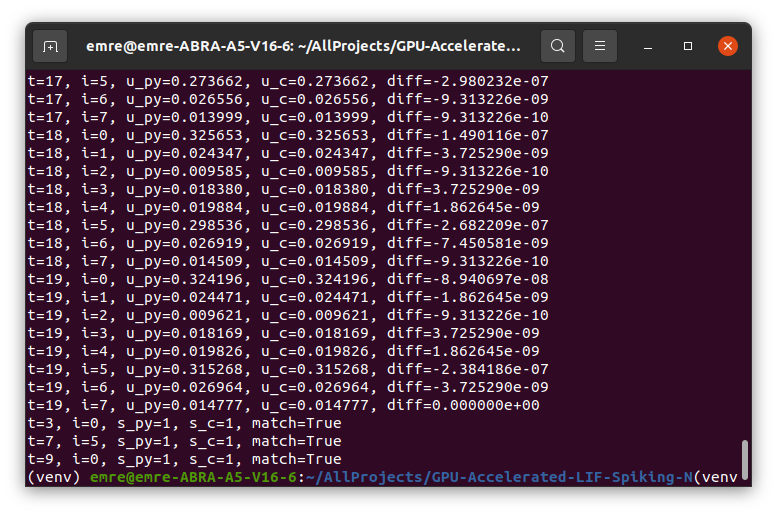
\includegraphics[width=0.48\textwidth]{comp_C_vs_torch.png}
  \caption{Comparison output of CPU and pytorch versions}
  \label{fig:comp_w_pytorch}
\end{figure}

\section{Basic GPU Model}

\subsection{Implementation}
The Basic GPU Model implementation is done after the CPU model, to have a middle ground before optimizing this version.

There are two separate kernels because there is a data dependency between the synapse and neuron update. 
The kernels need to be separate because the input current accumulation is done in the synapse update, and it is being used right after for the neuron update. 

The synapse kernel is given at the Figure\ref{fig:Synapse_Basic_GPU_impl}.
With the GPU version it is clearly visible that now there is only one for loop, compared to two for loops of the CPU model.

  \begin{figure}[h]
\centering
\begin{lstlisting}
  __global__ void synapse_kernel(...)
  {
      int i = blockIdx.x * blockDim.x + threadIdx.x;
      if (i >= n) return;

      // Accumulation
      float acc = (float)ext_step[i] * ext_w;

      // Adding recurrent input from all previous spikes.
      int row = i * n;
      for (int j = 0; j < n; ++j)
          acc += W[row + j] * (float)s_prev[j];

      // Decay 
      g[i] = alpha * g[i] + acc;
  }
\end{lstlisting}
\caption{Synapse Kernel of the Basic GPU implementation}
\label{fig:Synapse_Basic_GPU_impl}
\end{figure}

The neuron kernel is given at the Figure~\ref{fig:Neuron_Basic_GPU_impl}. After the kernel indexing is done, the membrane potential being updated and the spikes are being recorded.


  \begin{figure}[h]
\centering
\begin{lstlisting}
  __global__ void neuron_kernel(...)
  {
      int i = blockIdx.x * blockDim.x + threadIdx.x;
      if (i >= n) return;

      // Membrane Update (Soft Reset)
      float ui = u[i] - (float)s_prev[i] * thresh;
      ui = beta * ui + (1.0f - beta) * g[i];

      // Spike generation
      uint8_t si = (ui > thresh) ? 1 : 0;
      u[i] = ui;
      s[i] = si;
  }
\end{lstlisting}
\caption{Neuron Kernel of the Basic GPU implementation}
\label{fig:Neuron_Basic_GPU_impl}
\end{figure}

In this naive version, there are a couple of problems that are apparent. There is no kernel fusion; two seperate kernel introduces an overhead.
The for loop in the synapse kernel is sequential; no shared memory or tiling is used.

\subsection{Testing}
Testing for the basic GPU version is done with another script; 
at this step, a Python grapher script has been written to demonstrate the neuron parameters with respect to the timesteps.
Three different versions of the same SNN model with the same weights and external spikes are being compared: Python (torch), CPU, and GPU versions.

The best way to ensure that the SNN computations are correct and align with the Python (Torch) reference is to compare the membrane potential with respect to timesteps. 
In Figure~\ref{fig:membrane_comp_Torch_CPU_GPU}, spikes are happening in the correct timesteps and the membrane potentials are aligned perfectly.

\graphicspath{{images}}
\begin{figure}[H]
  \centering
  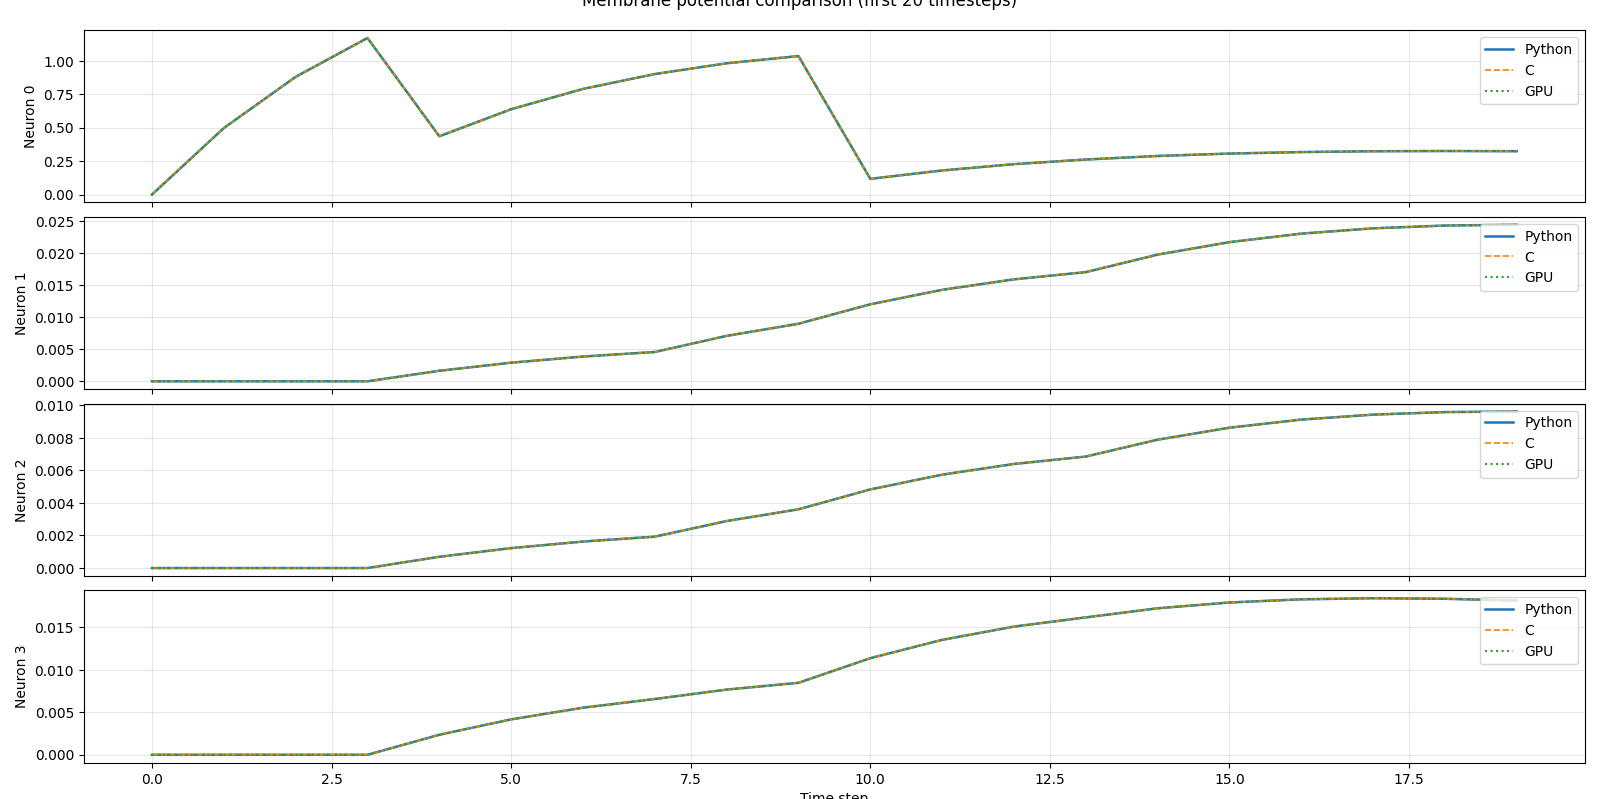
\includegraphics[width=0.48\textwidth]{Python_C_GPU_membrane_comparison.png}
  \caption{Membrane Potential comperison of Torch, CPU and GPU versions}
  \label{fig:membrane_comp_Torch_CPU_GPU}
\end{figure}

The next step is to show the absolute error of the GPU, how much it diverges from the reference. 
In Figure~\ref{fig:absolute_error_torch_GPU} absolute error of the first eight neurons being shown. 
The errors are zero for most of the neurons and almost zero for others; 
this small difference could be the result of the float representation difference between the different systems.

\graphicspath{{images}}
\begin{figure}[H]
  \centering
  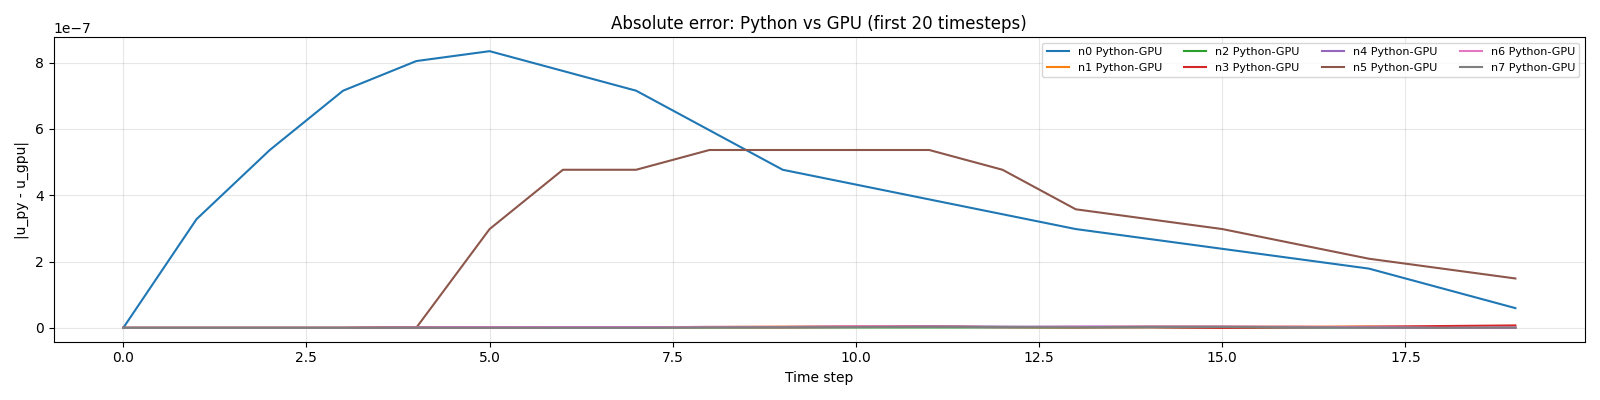
\includegraphics[width=0.48\textwidth]{Python_GPU_Absolute_error.png}
  \caption{Absolute error between the Torch and GPU versions}
  \label{fig:absolute_error_torch_GPU}
\end{figure}

\section{Optimized GPU Model}



\bibliographystyle{plain} % Styles: plain, unsrt, alpha, etc.
\bibliography{references}
\end{document}
